\documentclass[11pt]{article}

\usepackage{a4wide}
\usepackage[utf8]{inputenc}
\usepackage[russian]{babel}
\usepackage{graphicx}
\usepackage{amsmath}
\usepackage{amsfonts}
\usepackage{amssymb}
\usepackage{subcaption}
\usepackage{upgreek}
\usepackage{dsfont}
\begin{document}
	
	\thispagestyle{empty}
	
	\begin{center}
		\ \vspace{-3cm}
		
		
\includegraphics[width=0.5\textwidth]{msu.eps}\\
		{\scshape Московский государственный университет имени М.~В.~Ломоносова}\\
		Факультет вычислительной математики и кибернетики\\
		Кафедра системного анализа
		
		\vfill
		
		{\LARGE Курсовая работа}
		
		\vspace{1cm}
		
		{\Huge\bfseries <<Динамические системы и модели биологии>>}
	\end{center}
	
	\vspace{1cm}
	
	\begin{flushright}
		\large
		\textit{Студент 315 группы}\\
		А.\,В.~Бабаев
		
		\vspace{5mm}
		
		\textit{Научный руководитель}\\
		 Д.\,А.~Алимов
	\end{flushright}
	
	\vfill
	
	\begin{center}
		Москва, 2021
	\end{center}
	
	\newpage
	\tableofcontents
	\newpage
	{\vspace*{-2cm} \hspace*{-1cm}\section{Постановка задачи}}
	{Задана динамическая система:}
	\begin{equation}
		\begin{cases}
		\dot x = \frac{ax^2}{1 + x} - \frac{bxy}{1 + Ax},\\
		\dot y = -cy + \frac{dxy}{1 + Ax},
		\end{cases}
	\end{equation}  
	{где $a,b,c,d,A > 0$. Система рассматривается в $\mathds{R}_+^2.$ Необходимо:}
	{\begin{itemize}
			\item [1)]{Дать биологическую интерпретацию характеристик системы(хищник-жертва, характеристика трофической функции, очистка воды).}
			\item [2)]{Ввести новые безразмерные переменные, максимально уменьшив число входящих параметров. Выбрать два свободных параметра. Если число параметров больше двух, то считать остальные параметры фиксированными.}
			\item [3)]{Найти неподвижные точки системы и исследовать их характер в зависимости от значений параметров. Результаты исследования представить в виде параметрического портрета системы.}
			\item [4)]{Для каждой характерной области параметрического портрета построить фазовый портрет. Дать характеристику поведения системы в каждом из этих случаев.}
			\item [5)]{Исследовать возможность возникновения предельного цикла. В положительном случае найти соответствующее первое ляпуновское число. Исследовать характер предельного цикла(устойчивый, неустойчивый, полуустойчивый).}
			\item [6)]{Дать биологическую интерпретацию полученным результатам.}
	\end{itemize}}
	
	{\section{Биологическая интерпретация}}
	{Система (1) является системой типа <<хищник-жертва>>, в которой $x$ --- это численность жертв, а $y$ --- численность хищников. Основные предположения, положенные в основу данной системы характеризуются следующими гипотезами: в отсутствии хищников жертвы размножаются со скоростью $a \ (\dot{x} = \frac{ax^2}{1 + x})$; хищники в отсутствие жертв вымирают ($\dot{y} = -cy$); слагаемые, пропорциональные члену $xy$, рассматриваются как превращение энергии одного источника в энергию другого (эффект влияния популяции хищников на популяцию жертв заключается в уменьшении относительной скорости прироста численности жертв на величину, пропорциональную численности хищников); $\frac{d}{b}$ --- коэффициент переработки потребленной хищником биомассы жертвы в собственную биомассу.}
	{\section{Введение безразмерных переменных}}
	{Обозначим}
	\begin{equation}
	x = Bu(\tau), y = Cv(\tau), t = T\tau, \quad B,C,T - \text{константы}
	\end{equation}
	{замечая, что $\frac{d}{dt} = \frac{d}{d\tau}\frac{d\tau}{dt}=\frac{1}{T}\frac{d}{d\tau}$. Тогда}
	\begin{equation}
		\begin{cases}
		B\frac{1}{T}\frac{du}{d\tau} = \frac{aB^2u^2}{1 + Au} - \frac{bBuCv}{1 + ABu}\\
		C\frac{1}{T}\frac{dv}{d\tau} = -cCv + \frac{dBuCv}{1 + ABu}
		\end{cases}
	\end{equation}
	\newpage
	\[ \begin{cases}
		\frac{du}{d\tau} = \frac{aBu^2T}{1 + Au} - \frac{buCvT}{1 + ABu}  \\
		\frac{dv}{d\tau} = -cvT + \frac{dBuvT}{1 + ABu}
	\end{cases}  \]
	{Положим, что $B = 1, C = \frac{1}{bT}, T = \frac{1}{a}$:}
	\[ \begin{cases}
		\frac{du}{d\tau} = \frac{u^2}{1 + Au} - \frac{uv}{1 + Au}\\
		\frac{dv}{d\tau} = -\frac{c}{a}v + \frac{duv}{a(1 + Au)}
	\end{cases}  \]	
	{Сделаем замену: $-\frac{c}{a} = k, \frac{d}{a} = h.$ Получим:}
	\begin{equation}
		\begin{cases}
		\frac{du}{d\tau} = \frac{u^2}{1 + Au} - \frac{uv}{1 + Au}\\
		\frac{dv}{d\tau} = kv + \frac{huv}{1 + Au}
		\end{cases}
	\end{equation}
		   
	{\section{Неподвижные точки системы}}
	{\subsection{Нахождение неподвижных точек}}
	{\textbf{Определение 1.} Точка $a \in \mathbb{R}^n$ называется неподвижной точкой динамической системы $\dot{x}_i = f_i(x_1,\ldots,x_n),$ где $(x_1,\ldots,x_n) \in D \subset \mathbb{R}^n, i = \overline{1,n}, f = (f_1, \ldots, f_n),$ если $f(a) = 0$.}
	\newline
	{Воспользуемся определением, чтобы найти неподвижные точки:}
	\begin{equation}
	\begin{cases}
				\frac{u^2}{1 + Au} - \frac{uv}{1 + Au} = 0,\\
				kv + \frac{huv}{1 + Au} = 0.
	\end{cases}
	\end{equation}
	{Очевидно, что $u = 0, v = 0$ --- неподвижная точка. Далее положим, что $u^2 + v^2 > 0:$}
	\[ \frac{u - v}{1 + Au} = 0, \]
	\[ u = v, \]
	{Подставим во второе уравнение:}
	\[  kv + \frac{hv^2}{1 + Av} = 0, \]
	\[ (Ak + h)v^2 + kv = 0, \]
	\[v = -\frac{k}{Ak + h}. \]
	{Таким образом, в системе присутствуют одна или две неподвижные точки:}
	\begin{itemize}
		\item [1)]{$O$ с координатами $u = 0, v = 0,$}
		\item [2)]{$M$ с координатами $u = -\frac{k}{Ak + h}, v = -\frac{k}{Ak + h}$ (возникает только при $Ak + h > 0$. В противном случае система содержит только одну неподвижную точку).}
	\end{itemize}
	\newpage
	{\subsection{Характер неподвижных точек}
	{Пусть задана динамическая система с непрерывным временем:}
	\begin{equation}
	\dot{u} = f(u), \quad u \in U \subseteq \mathbb{R}^n, \quad f:U \rightarrow \mathbb{R}^n.
	\end{equation}
	{Предположим, что $u^*$ --- положение равновесия этой системы. Обозначим $J(u^*)$ матрицу Якоби вектор-функции $f(u)$ в точке $u^*$. Пусть $n_+, n_0, n_-$ --- число собственных значений $J(u^*)$ (с учетом кратности) с положительной, равной нулю и отрицательной вещественной частью соответственно.}
	\newline
	\newline
	{\textbf{Определение 2.} Положение равновесия динамической системы (5) называется $\textit{гиперболическим}$, если $n_0 = 0,$ т.е. не существует собственных чисел, расположенных на мнимой оси. Гиперболическое положение равновесия называется $\textit{гиперболическим седлом},$ если $n_+n_- \neq 0.$ } 
		\newtheorem{theorem}{Теорема}
	\begin{theorem}
	{(А.М. Ляпунов, А. Пуанкаре). Пусть $u^*$ --- гиперболическое положение равновесия (6). Тогда, если $n_+ = 0,$ то положение равновесия $u^*$ асимптотически устойчиво; если $n_+ > 0$, то неустойчиво.}
	\end{theorem}		
	{Выпишем матрицу Якоби для данной системы (4):}
	\begin{equation}
		J(u,v) = \begin{pmatrix}
		\frac{(-v + 2u)(Au + 1) - (u^2 - uv)A}{(Au + 1)^2}	& -\frac{u}{1 + Au} \\
			\frac{hv}{(1 + Au)^2}& k + \frac{hu}{1 + Au}
		\end{pmatrix}
	\end{equation}
	{Рассмотрим ее сначала в точке $O$, потом --- в точке $M$:}
	\begin{equation}
	J(O) = \begin{pmatrix}
	0 & 0 \\
	0 & k
	\end{pmatrix}
	\end{equation}
	\begin{equation}
	det(J(O) - \lambda I) = det\begin{pmatrix}
	-\lambda & 0 \\
	0 & k - \lambda
	\end{pmatrix} = \lambda^2 - \lambda k= 0.
	\end{equation}
	{Получаем, что $\lambda_1 = 0, \lambda_2 = k.$ Заметим, что одно из собственных значений нулевое, то есть лежит на мнимой оси, поэтому данное положение равновесия не является гиперболическим, и теорема 1 неприменима. }
	\newline
	\newline
	\begin{center}
		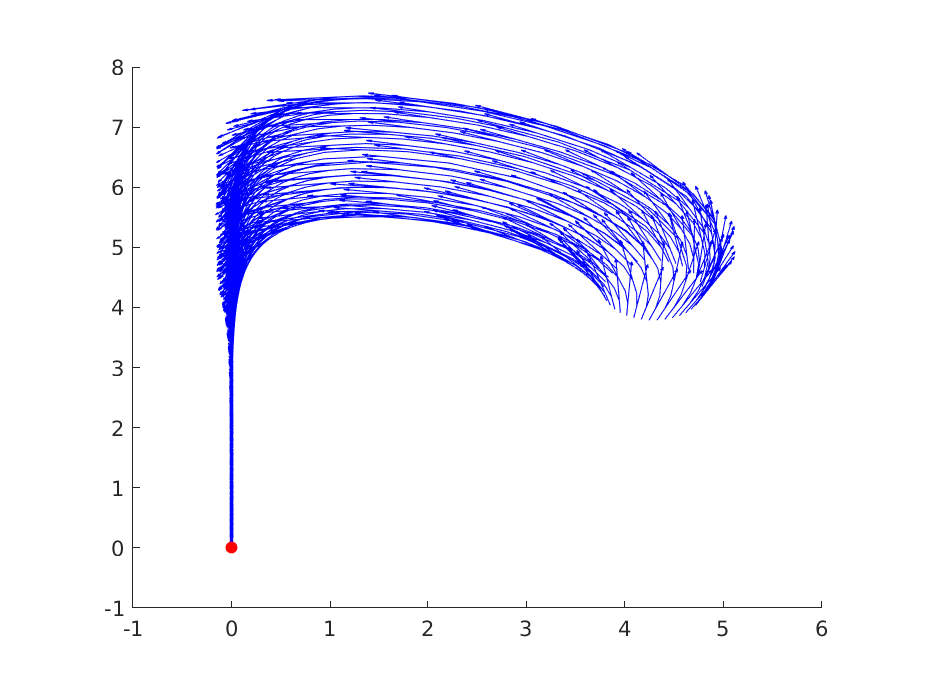
\includegraphics[width=0.7\textwidth]{pic_1.eps}\\
		{Рис. 1. Зависимость $u(v).$ Поведение траекторий вблизи положения равновесия (0,0) при значения параметров $A = 0.1, k = -0.2, h = 0.6.$ }
	\end{center}
	{Рассмотрим в точке $M =(-\frac{k}{Ak + h}, -\frac{k}{Ak + h})$:}
	\begin{equation}
	J(M) = \begin{pmatrix}
	-\frac{k}{h} & \frac{k}{h} \\
	-\frac{k}{h}(Ak + h) & 0
	\end{pmatrix}
	\end{equation}
	\begin{equation}
	det(J(M) - \lambda I) = det\begin{pmatrix}
	-\frac{k}{h}-\lambda & \frac{k}{h} \\
	-\frac{k}{h}(Ak + h) & -\lambda
	\end{pmatrix} = \lambda^2 + \frac{k}{h}\lambda + \frac{k^2}{h^2}(Ak + h) = 0.
	\end{equation}
	\begin{equation}
	   D = \frac{k^2}{h^2} - 4 \frac{k^2}{h^2}(Ak + h). 
	\end{equation}
	
	{Тогда корнями будут:}
	\begin{equation}
		\lambda_{1,2} = \frac{-\frac{k}{h} \pm \frac{|k|}{h}\sqrt{1 - 4(Ak + h)}}{2}
	\end{equation}
	{Заметим что параметр $k < 0$ а параметр $h > 0$. Из этого следует что $\frac{k}{h}$ принимает отрицательное значение. Так же получаем, что положения равновесия системы являются гиперболическими. Рассмотрим случаи:} 
	\begin{equation}
		D \geq 0 \Leftrightarrow 1 - 4(Ak + h) \geq 0
	\end{equation}
	{Имеем, что $\lambda_{1,2}$ вещественные числа. Положение равновесия --- узел, при $\frac{1}{4} > Ak+h > 0$. По теореме 1 получается неустойчивый узел.}
	\begin{equation}
	D < 0 \Leftrightarrow 1 - 4(Ak + h) < 0
	\end{equation}
	{Тогда $\lambda_{1,2}$ --- комплексные с положительной вещественной частью(которые совпадают), значит положение равновесия есть фокус. Но, согласно ограничению на константы $Ak + h < 0$ следовательно такой ситуации в нашей системе возникнуть не может.}
	\newline
	{Рассмотрим неустойчивую узловую точку при значении параметров $A = 0.1, k = -0.6, h = 0.2.$ Получим неустойчивый узел в точке $M = (4.2857,4.2857).$}
	\begin{center}
		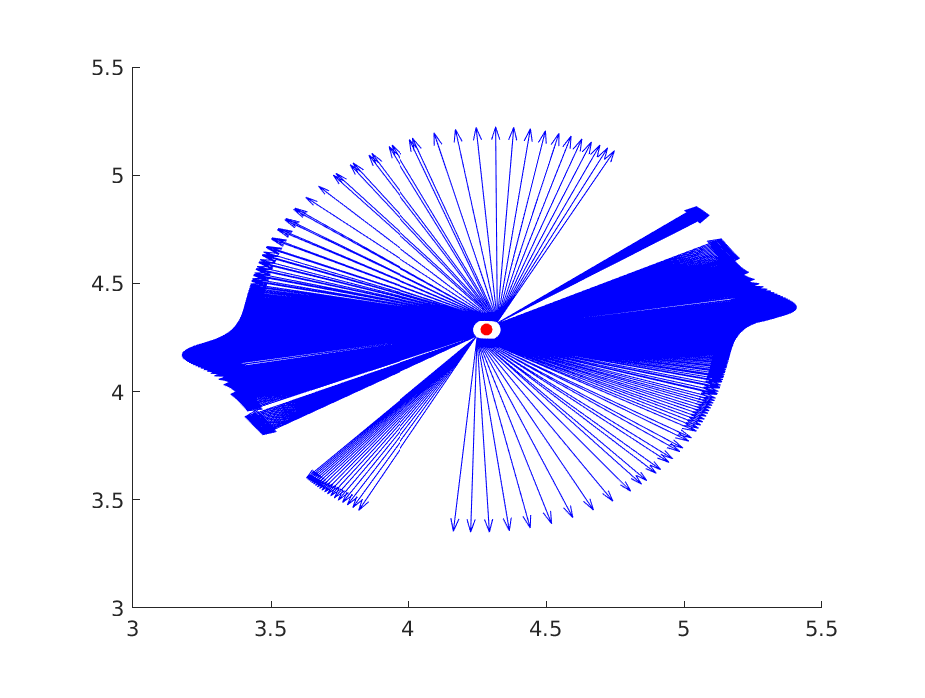
\includegraphics[width=0.7\textwidth]{pic_2.eps}\\
		{Рис. 2. Зависимость $u(v).$ Поведение траекторий вблизи положения равновесия (4.2857,4.2857) при значения параметров $A = 0.1, k = -0.6, h = 0.5.$ }
	\end{center}
	\newpage
	{\section{Предельные циклы}}
	{Рассмотрим динамическую систему:}
	\begin{equation}
		\dot{u} = f(u), \quad u \in U \subseteq \mathbb{R}^n, \quad f:U \rightarrow \mathbb{R}^n
	\end{equation}
	{\textbf{Определение 3.} Решение $u(t)$ задачи (16) называется \textit{периодическим} с периодом $T > 0,$ если $u(t + T) = u(t)$ для любого $t$, период $T$ --- наименьшее из таких чисел, для которых выполняется последнее равенство.} 
	\newline
	\newline
	{\textbf{Определение 4.} Замкнутую траекторию $\gamma(u_0)$ системы (16) будем называть \textit{предельным циклом}, если в окрестности этой траектории не других замкнутых орбит.}
	\newline
	\newline
	{\textbf{Определение 5.} Бифуркация положения равновесия, соответствующая появлению собственных чисел $\lambda_{1,2} = \pm i \omega_0, \omega_0 > 0,$ называется бифуркацией \textit{Пуанкаре-Андронова-Хопфа} или \textit{бифуркацией рождения цикла}.}
	\newline
	\newline
	{В предыдущем пункте при нахождении собственных значений мы убедились, что ни для каких допустимых значений параметров не возникают собственные значения с действительной частью, равной нулю, то есть целиком лежащие на мнимой оси. Из этого следует, что бифуркация рождения цикла в данной системе невозможна, и предельных циклов нет.}
	\newpage	
	{\vspace*{-2cm} \hspace*{-1cm}\section{Биологическая интерпретация}}
	Если рассмотреть полученные графики, можно провести биологическую интерпретацию полученных результатов. В частности, мы видим, на рисунке 1, что сначала происходит гибель жертв и одновременный рост хищников, однако спустя некоторое время, хищники так же вымирают. Наличие неустойчивого узла при определенных параметрах гласит о том, что "раскручивается спираль" хищников и жертв, которая, в конечном счете, привет их к гибели. 
	\newpage
	{\vspace*{-2cm} \hspace*{-1cm}\section{Cписок литературы}}
	{\hspace*{-0.6cm}[1]Алимов Д.А., лекции и семинары "Динамические системы и биоматематика". ВМК МГУ, Москва, 2021.}
	\newline
	{[2] Братусь А.С., Новожилов А.С., Платонов А.П. "Динамические системы и модели биологии".}
\end{document}